
\chapter{InSAR Background}
\label{CHAP:3}

In this chapter...

%Simons: operating at microwave frequencies, synthetic aperture radar (SAR) systems provide unique images representing the electrical and geometrical proper- ties of a surface in nearly all weather conditions. Since they provide their own illumination, SARs can image in daylight or at night. 

%https://www.usgs.gov/observatories/yvo/news/insar-magic-deformation-camera-no-one-saw-coming
%Tracking radars "ping" a target, record the reflected signal, and measure (1) how long it took for the ping's round trip, and (2) the frequency of the return signal. The travel time is a measure of distance to the target. The target's velocity can be determined from the frequency of the return signal, which differs from that of the transmitted signal as a result of the Doppler effect (this is the effect that makes a siren sound different when it is coming toward you versus moving away from you, for example). Air traffic control radars and police speed detectors work on this principle.

\section{Radar Imaging}
\label{CHAP:3-radar}

``Radar'' was originally an acronym for ``RAdio Detection And Ranging'' but it has since become ubiquitous enough enter the common vernacular. Unlike passive sensors that rely on illumination for outside sources, such as optical cameras, a radar is an active sensor that emits its own electromagnetic energy. 
As such, radars are able to operate both day and night, and generally operate at microwave frequencies that are not blocked by clouds (around between 1 GHz and 300 GHz, or wavelengths of 3 m to 1 mm).
%The ability to operate both day and night is one of the main advantages of radar.

The original radars developed during World War 2 were for tracking the position of targets. In these systems, the range to the target is calculated from the round trip travel time of an electromagnetic pulse that is reflected off the target, and the angle is determined by the antenna pointing direction.
%system emits pulses of electromagnetic energy and detects the time delay of their return, which can be converted to a range using the speed of light. 
Later researchers developed imaging radar systems converted a series of radar pulses on a moving platform into a two-dimension image. Although these images originally had coarse resolution, research led by Carl Wiley at Goodyear in the 1950s resulted in the development of the radar imaging technique known as synthetic aperture radar (SAR) \citep{Wiley1954PulsedDopplerRadar, Wiley1985SyntheticApertureRadars}.
%Since electromagnetic waves get scattered by objects that are roughly the size of their wavelength, this means that radars are not blocked by water droplets and may see through clouds.
%At Goodyear in the 1950s, Carl Wiley developed the concept of the synthetic aperture \citep{Wiley1954PulsedDopplerRadar}, which was the start of the radar imaging technique known as synthetic aperture radar (SAR) \citep{Wiley1985SyntheticApertureRadars}.
The first demonstration of a spaceborne earth-observing SAR mission with interferometric capability was Seasat, launched by NASA in 1978
%equipped with an L-band radar 
\citep{Born1979SeasatMissionOverview, Gabriel1989MappingSmallElevation}.
Since that time, there have been dozens of mission launched by various space agencies, leading some to call the last decade ``the golden age of SAR'' \citep{Moreira2014GoldenAgeSpaceborne}.

%Synthetic aperture radar (SAR) is a powerful radar imaging technique which works day and night through all weather conditions.



\subsection{Timeline of SAR Constellations}



\begin{figure}
	\centering
	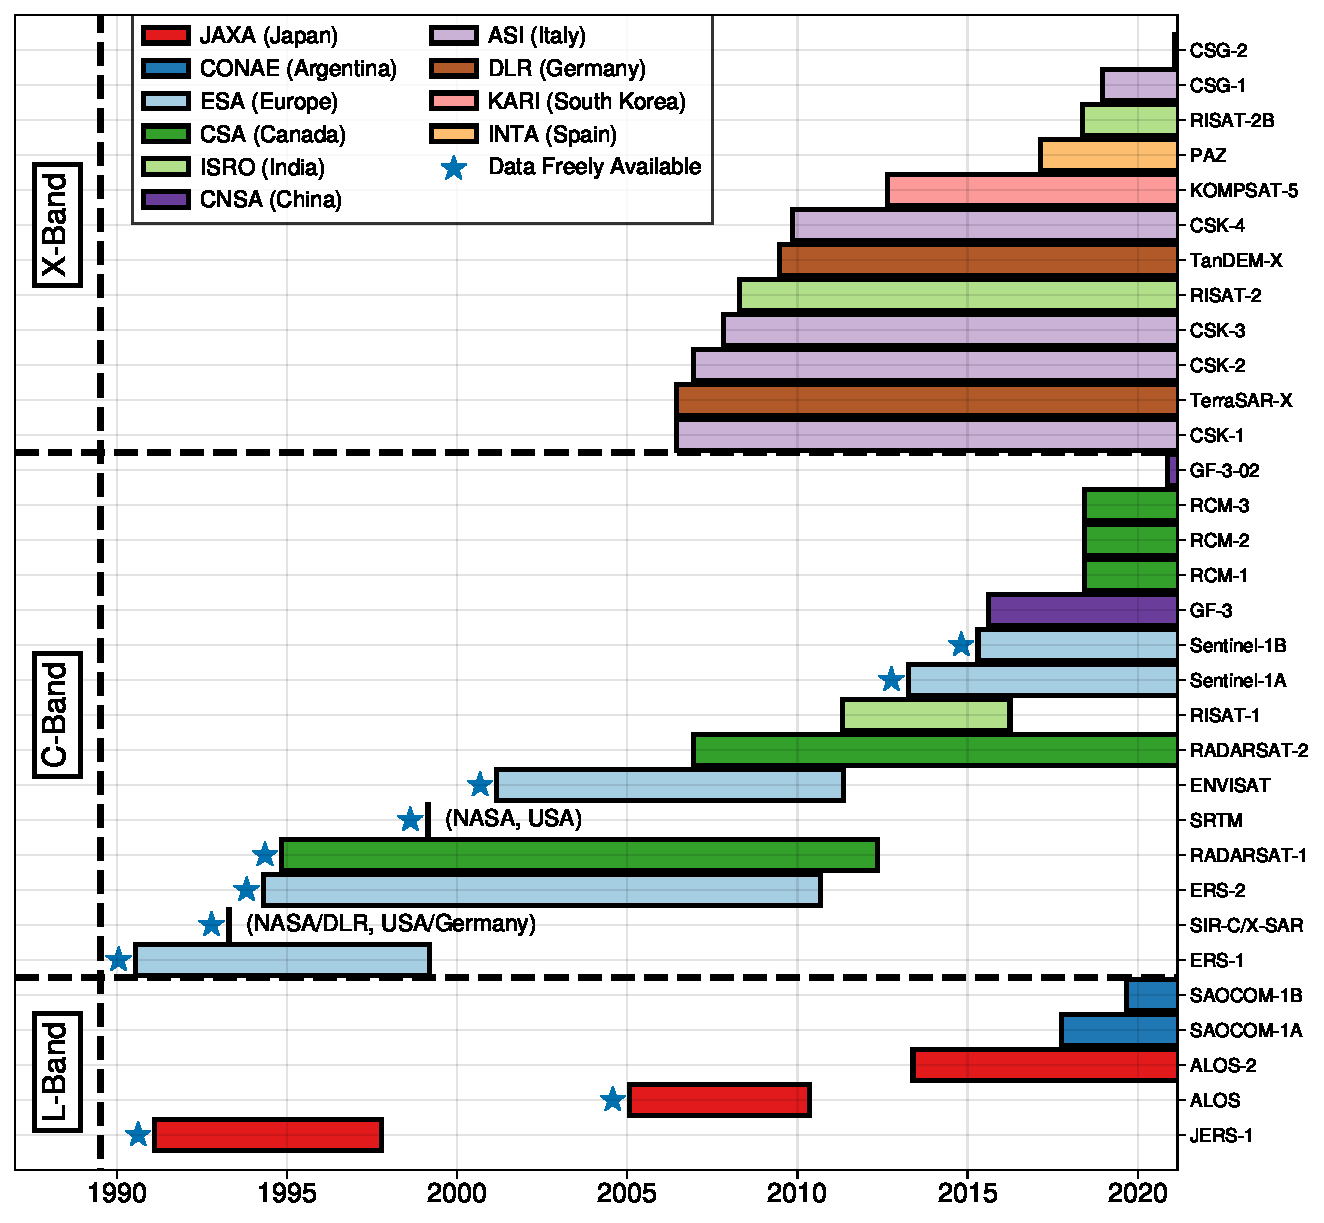
\includegraphics[width=1.1\textwidth]{figures/chapter3-sar/sar-missions.pdf}
	\caption[Timeline of government SAR missions]{Timeline of government-sponsored SAR missions since 1990. Bar lengths indicate life span of mission. Bars which intersect the right edge indicate ongoing missions.
		Colors indicate the space agency operating the mission.
		Missions which provide data free of charge to the general public (as of May 2022) are marked with blue stars.
		Vertical sections of the timeline are divided by the radar frequency of the sensor, showing (from top to bottom) the X-band, C-band, and L-band missions.
		Note that SIR-C/X-SAR and SRTM were equipped with both C- and X-band sensors.}
	\label{fig:ch3-sar-missions}
\end{figure}


Figure \ref{fig:ch3-sar-missions} shows a timeline of SAR missions that have been launched by governments and space agencies since 1990. The missions are grouped vertically into the three most commonly used frequency bands for SAR sensors in earth-observing missions: L-band (wavelengths of $\sim$24 cm), C-band ($\sim$6 cm cm) and X-band ($\sim$3 cm).
During the 90s, the European Space Agency (ESA) launched two C-band SAR satellites: ERS-1 in 1991 and ERS-2 in 1995. The ERS-1 satellite provided the first practical demonstration of spaceborne InSAR's ability to capture surface deformation
when \cite{Massonnet1993DisplacementFieldLanders} mapped the  surface deformationn pattern caused by the 1992 Landers, California earthquake. The first L-band SAR satellite, JERS-1, was launched by NASDA\footnote{Although JERS-1 is labeled as a JAXA mission in Figure \ref{fig:ch3-sar-missions}, it was run by NASDA at the time. In 2003, NASDA merged with two other Japanese space agencies, ISAS and NAL, to form JAXA.} in 1992, and the Canadian Space Agency (CSA) launched their own C-band mission, RADARSAT-1, in 1995.


The most influential SAR mission within the science community has been Sentinel-1 \citep{Torres2012GmesSentinel1}. First launched in 2014, the Sentinel-1 satellites acquire data using an imaging mode that allow them to image very large swaths ($\sim$240 km wide in the interferometry mode) \cite{Zan2006TopsarTerrainObservation}, allowing them revisit any point on Earth every 12 days. 
Additionally, Sentinel is the first mission of it's kind to provide it's data for free, leading to a transition from using SAR and InSAR in opportunistic experiments to being able to operationally monitor nearly anywhere on Earth  \cite{Rosen2021ShiftingGround}.
Currently Sentinel-1 is the only ongoing mission with open SAR data; however, the future launch of the NISAR ISRO SAR mission (NISAR) will also provide free L-band SAR data with global coverage \citep{Rosen2015NasaIsroSar}.


\begin{figure}
	\centering
	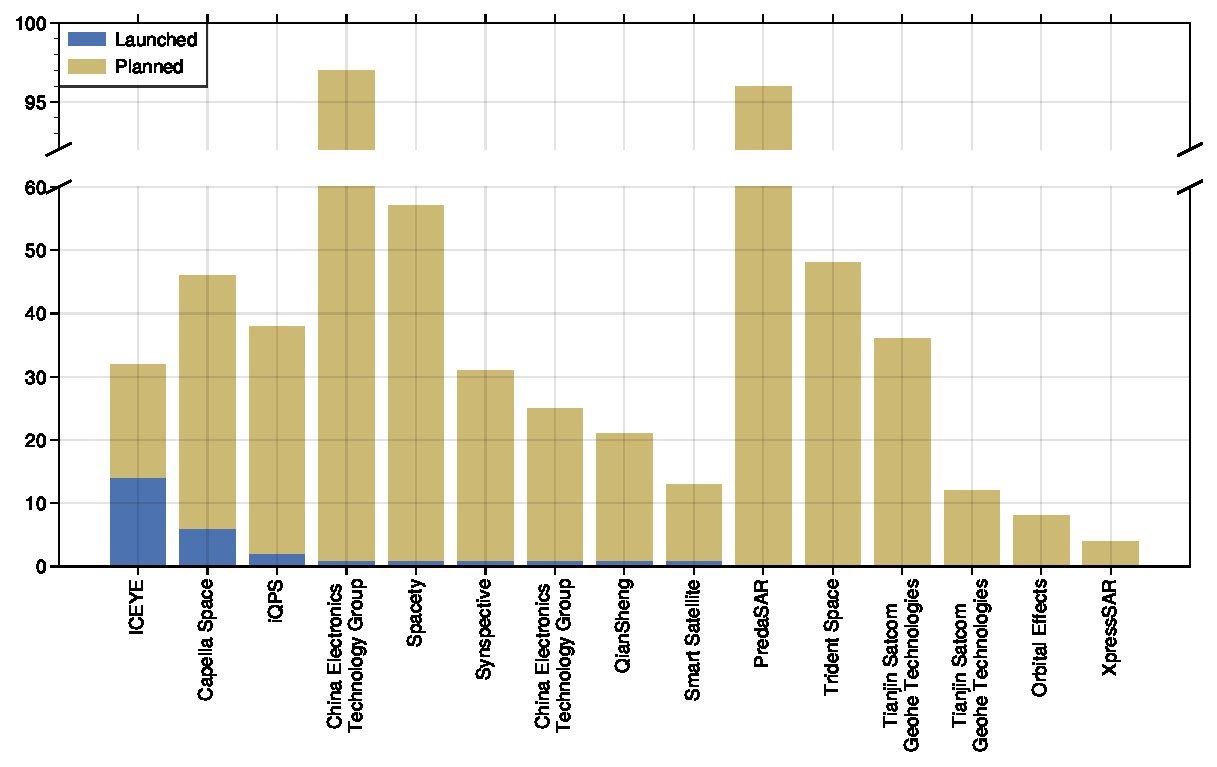
\includegraphics[width=1.0\textwidth]{figures/chapter3-sar/sar-private-constellations.pdf}
	\caption[Private sector SAR constellations]{SAR constellations run by private companies, showing the number of currently launched satellites (blue) stacked under the number of future planned launches (gold). Note the broken y-axis scale, as two companies 
		%	(China Electronics Technology Group and PredaSAR) 
		are planning constellations of 96 satellites.
	}
	\label{fig:ch3-sar-private-const}
\end{figure}



The first small SAR SmallSats (satellites weighing under 180 kg) have been launched by private companies over the past four years (Figure \ref{fig:ch3-sar-private-const}). Finland's ICEYE had its first succesful launch in January 2018, while Capella Space had their first launch 11 months later. Seven other companies have since launched at least 1 SAR satellite, and in the next five years, there are plans to launch over 500 additional SAR SmallSats \citep{Kulu2021SatelliteConstellations2021}. While many large SAR constellations expect sub-hourly revisit time for any given point on earth \citep{Stringham2019CapellaXband}, only the large government SAR missions, such as Sentinel-1, ALOS, and NISAR, explicitly plan for consistent global coverage in their mission objectives. However, the possibility of daily or hourly InSAR revisit times opens many new applications previously not possible with the 6-12 day revisit times of large SAR missions \citep{YagueMartinez2021TowardsFrequentFlood, Taylor2021RemoteSensingMountain, Kitajima2021PotentialSarSmall}.






\section{Synthetic Aperture Radar}
\label{CHAP:3-sar}


Synthetic aperture radar is an imaging technique that uses a pulsed radar mounted on a moving platform. A two-dimensional image is created by coherently processing the returned energy pulses. While the images are often displayed in grayscale and may appear similar to optical images, they represent the electrical and geometrical properties of the objects in the scene \cite{Simons2007InterferometricSyntheticAperture}.
%To create a radar image, the energy scattered by points on the ground must be collected and focused in two dimensions.  The image represents the electrical and geometrical properties of the scene \cite{Simons2007InterferometricSyntheticAperture} 


The SAR imaging geometry is shown in Figure \ref{fig:ch3-sar-geometry}. A side-looking radar on a platform at height $h$ moves in the azimuth directory $x$ at a velocity $v$.  The radar repeatedly emits pulses at some interval (called the \emph{pulse repetition interval}, or PRI) that travel in the range direction.
%The illuminated portion of the ground has a swath width of $r \lambda / w$
%The width of the swath for stripmap operation is controlled by the antenna width, $w$, as $r \lambda / w$. Likewise, the size of the illuminated swath in the along track direction is $r \lambda / L$.
The line of sight (LOS) vector is defined as the unit vector pointing from the radar antenna to a point in the illuminated ground swath.
Each pulses illuminates a portion of the ground, known as the radar footprint.


\begin{figure}
	\centering
		\includegraphics[width=0.99\linewidth]{figures/chapter3-sar/ch3-sar-geometry.pdf}
	\caption[Acquisition geometry of an imaging radar]{Acquisition geometry of an  imaging radar. A platform containing a radar instrument is moving with speed $v$ in the azimuth/along-track direction, $x$ at a height $h$.
    The slant range $r$ to the ground point is measured along the line-of-sight (LOS) direction from the antenna to the ground.
   	The radar antenna here has length $L$ (in the azimuth direction) and width $w$.
   	As the radar sends out pulses, each one into an area on the ground called the beam ``footprint'' (oval shape). 
%   	As the platform moves and sends more pulses, they sweep out the radar swath (gray region).
	}
	\label{fig:ch3-sar-geometry}
\end{figure}

% Resolution: shorter pulse better resolution, but also lowers SNR. To get around tradeoff, send long with LFM chip to high snr and fine resolution in range direction
%

The signal to noise ratio (SNR) of the system depends on the total energy transmitted.  SNR can be increased by either sending a higher peak power (which is often limited by design constraints) or sending a pulse of longer duration $\tau$. This presents a dilemma: sending pulses with a larger $\tau$ results in coarser range resolution $\delta_r$, where resolution is the ability to distinguish scatters illuminated by the same radar pulse. In the absence further processing, the resolution in range would is $\delta_r = \frac{c \tau}{2}$, where $c \approx 3 \times 10^8$ is the speed of light. Thus, a pulse with $\tau = 30 $ microseconds would have about a 4.5 km resolution.

However, SAR systems usually transmit pulsed waveforms called \emph{chirps} whose frequency $f$ increases over time. For example, in a linear frequency moduled (LFM) chirp, the frequency can be written as 
\begin{equation}
	f(t) = k t
\end{equation}
where $k$ is the chirp slope (in Hz / s) and $-\tau / 2 < t < \tau/2$.
These special waveforms allow the receiver to correlate the returned echoes with a \emph{matched filter}, or a replica of the transmitted chirp. The new range resolution after using the matched filter depends on the frequency bandwidth, $BW$, of the chirp:  $BW = f_{max} - f_{min}$.
improves the range resolution to $\delta_r = \frac{c}{2 BW}$, where is the frequency bandwidth of the chirp. 


Figure \ref{fig:ch3-range-compress} demonstrates the effect of using chirped waveforms on range resolution using an example chirp with parameters matching the ERS-1 satellite (Figure \ref{fig:ch3-range-compress}a).
%The real part of an example chirp with parameters matching the ERS-1 satellite has an oscillation frequency which increases linearly over time (Figure \ref{fig:ch3-range-compress}a). 
The chirp has a duration of $\tau \approx 37.12 \mu s$, a chirp slope $k$ of $4 \times 10^{11} Hz / s$, resulting in frequency bandwidth $BW = k \tau$ $\approx$15.5 MHz (Figure \ref{fig:ch3-range-compress}b). By correlating the transmitted chirp with its complex conjugate, we get the impulse response of a point scatter (Figure \ref{fig:ch3-range-compress}c). If a chirp with the same time duration had a smaller slope $k$ (Figure \ref{fig:ch3-range-compress}d), the bandwidth would shrink by the same proportion (Figure \ref{fig:ch3-range-compress}e), and the impulse response would also be more spread out (Figure \ref{fig:ch3-range-compress}f).
Thus, we see that using chirped waveforms reverses the original problem, as a pulse with larger bandwidth actually has better resolution than a shorter pulse.


\begin{figure}
	\centering
%	\includegraphics[width=0.99\linewidth]{figures/chapter3-sar/ch3-range-compress.pdf}
	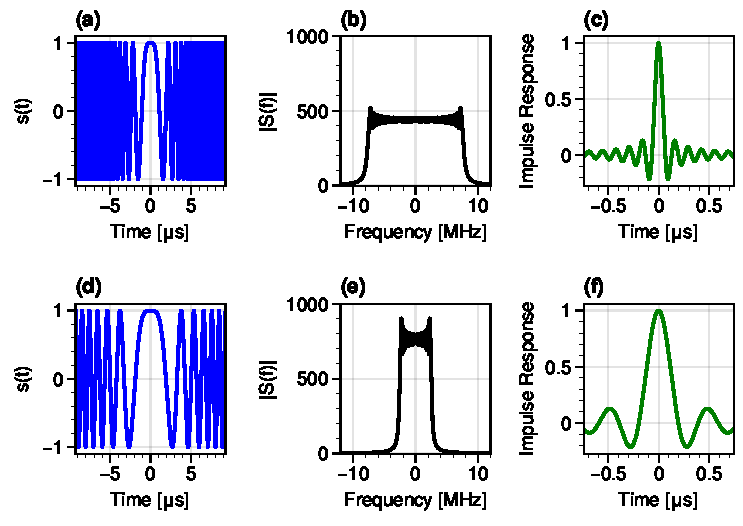
\includegraphics[width=0.99\linewidth]{figures/chapter3-sar/radar-chirp-bandwidth-ers.pdf}
%		\includegraphics[width=0.99\linewidth]{figures/chapter3-sar/radar-chirp-bandwidth-ers2.pdf}
	\caption[Range resolution from chirp compression]{
		(a) The real part of a linear frequency-modulated chirp with a duration of $\tau \approx 37.12 \mu s$ and a chirp slope $k = 4 \times 10^{11} Hz / s$.
		(b) The magnitude of the Fourier transform of the chirp is approximately a rectangle function, which shows the chirp bandwidth $BW = k \tau$ $\approx 15.5$ MHz.
		(c) Matched filtering of the returned echo from one point scatterer yields the impulse response, which shows the approximate 10 meters of range resolution (or $\sim$65 ns in time).
		(d) For a chirp with the same slope $k$ and 1/3 the duration $\tau$ the frequency bandwidth is also cut by 1/3 (e), the corresponding impulse response (f) and range resolution is 3 times worse.
	}
	\label{fig:ch3-range-compress}
\end{figure}


In the azimuth direction, the size of the radar footprint determines which ground points can be distinguished from the echo of one pulse;  this is known as the \emph{real aperture radar} (RAR) resolution. The footprint size can be written as $r \lambda / L$, which comes from the antenna's angular beam width of $\lambda / L$ and the range $r$ to the target. The earliest radar imaging platforms were limited to this resolution in azimuth. For an airborne platform with a 1 meter antenna imaging at C-band, this would be a $\sim$600 meter resolution. Note that for some applications, such as military detection applications or wide-area ocean mapping \cite{Simons2007InterferometricSyntheticAperture}, this azimuth resolution is sufficient; however, the RAR resolution for spaceborne radars are on the order of 10s of kilometers, which is far too coarse for most applications.


%The advantages long wavelengths offer in terms of penetration come with compensating drawbacks. The resolution a sensor depends on the wavelength and on the size of its aperture—the mirror or lens in the case of a camera or a telescope, the antenna in a radar. If you lengthen the wavelength, you increase the size of the aperture you need in order to achieve a given resolution. To produce detailed images with radar requires a very large aperture indeed—far larger than anything a single spacecraft can offer.

%> Synthetic-aperture radar (SAR) provides a way round that problem. Satellites move at quite a clip—typically, in low orbit, around 25,000kph. By taking all the echoes a radar satellite gets from a given target as it passes over it—and processing them into a single image, SAR produces a result as precise as if it had been made using a single aperture as wide across as the distance the satellite travelled while gathering the data—tens of hundreds of kilometres (see diagram).
The resolution in azimuth can be greatly improved by creating a \emph{synthetic aperture}, which is a technique that processes the reflected echoes coherently (i.e. using both magnitude and phase) to focus the image (Figure \ref{fig:ch3-synth-aper}).
%where the energy from a series of pulse returns from a point target is coherently added.
Coherent processing is possible by carefully tracking each target's phase history, $ \phi(t) $, which is related to the range to the target $r(t)$ by $\phi(t) = -\frac{4 \pi}{\lambda} r(t)$.
There are multiple image formation algorithms which create this synthetic aperture and use the phase history. One of the first developed and most widely today used is the range-Doppler algorithm (RDA) \citep{Wu1976DigitalSystemProduce, Cumming1979DigitalProcessingSeasat}. 
RDA uses the apparent shift in Doppler frequency due to the platform motion to create a matched filter in azimuth, similar to the matched filter used for range compression.
%RDA is a frequency-domain algorithm, since it converts the phase history 
%Which converts the range-compressed data into the frequency domain. 
An alternative to RDA is time-domain backprojection \citep{Duersch2013BackprojectionSyntheticAperture}, which provides a more exact phase compensation at the cost of being more computationally expensive.
The backprojection algorithm collects the energy from every radar pulse containing a pixel after compensating for the range-dependent phase.
The complex-valued radar image $I$ for the pixel at location $ (x, y) $ can be formed by summing over all pulses:
\begin{equation}
	I(x, y) = \sum_{k} s(r(x, y, k)) e^{-j \frac{4 \pi}{\lambda} r(x, y, k)}
\end{equation}
where $j = \sqrt{-1}$, $r(x, y, k)$ is the range distance from the radar sensor to the point $ (x, y) $ at the time of the $k$th pulse, and $s(r)$ is the value of the returned pulse at the given range \citep{Zebker2018InsarMissionLevel}.
Thus, if the radar imaging geometry is known precisely, the coherent summation can be performed to focus the SAR image.

For any of the image formation methods, the final achievable azimuth resolution $\delta_{az}$ is
%Processing all echoes coherently results in a fine resolution in the azimuth direction, which is equal to the resulting that would be attainable only by a real aperture of length $2 L_s$ \citep{Cumming2004DigitalProcessingSynthetic}.
%The phase of each return echo at a time $t$ is related to the range $r$ by $\phi(t) = -\frac{4 \pi}{\lambda} r(t)$.
\begin{equation}
	\delta_{az} = \frac{L}{2}
\end{equation}
Note the this final resolution is independent of wavelength, range or platform speed,
Normal spaceborne satellites have antennas on the order of 5-10 meters, resulting in a $\delta_{az} $ between 2.5-5 meters.
The intuition behind this surprising result is that, unlike with RAR, a smaller physical antenna size $L$ leads to a wider angular beam width $ \lambda / L$. This means that a given target is illuminated for a longer time, leading to a greater number of pulses to coherently process. Thus, the azimuth resolution will actually improve with a smaller antenna size.

\begin{figure}
	\centering
	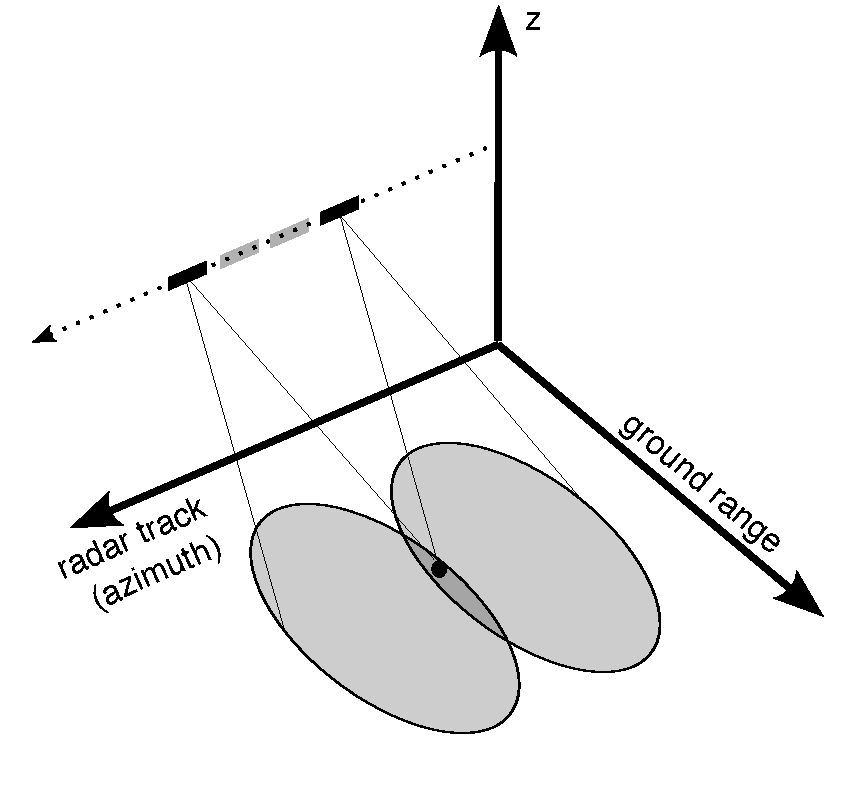
\includegraphics[width=0.8\linewidth]{figures/chapter3-sar/ch3-synth-aper2.pdf}
	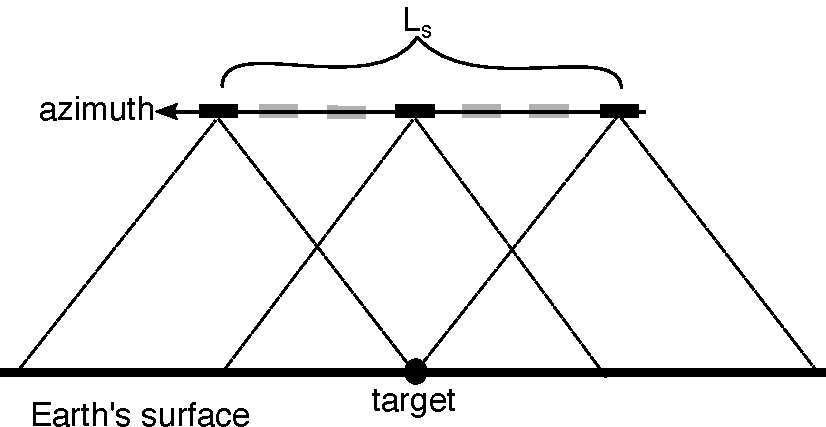
\includegraphics[width=0.99\linewidth]{figures/chapter3-sar/ch3-sar-synthetic-aperture.pdf}
	\caption[Concept of the synthetic aperture ]{Concept of the synthetic aperture.
	(Top) One point on the ground is illuminated by a series of pulses. Pictured here are the footprints of the first and last pulses that illuminate the point. 
	(Bottom) Side view of the pulses illuminating the target, forming a synthetic aperture of length $L_s$.
	}
	\label{fig:ch3-synth-aper}
\end{figure}



\section{SAR Interferometry}

SAR interferometry (or InSAR) refers to a broad class of applications that exploit the phase difference between two SAR images to derive new information; the most common applications are generating topography maps \cite{Graham1974SyntheticInterferometerRadar, Zebker1986TopographicMappingInterferometric, Gabriel1989MappingSmallElevation} and detecting surface deformation (\cite{Li1990StudiesMultibaselineSpaceborne, Massonnet1993DisplacementFieldLanders, Rosen2000SyntheticApertureRadar}). For topography mapping, two SAR antennas separated by a distance in the across-track direction are operating simultaneously (Figure \ref{fig:ch3-insar-geometry}a). The baseline causes the two radars to view the same point on the ground with a slight change in angle, which causes a difference in phase.
This phase difference is related to a geometrical path difference between the two radars which changes with topography. Thus, with precise knowledge of the viewing geometry, the phase can be converted to an altitude for each point in the SAR images 
The phase difference can be thought of as a third measurement, in addition to the location in the azimuth and range directions, that allows a reconstruction of the 3D location of the point \cite{Simons2007InterferometricSyntheticAperture}.

In repeat-pass InSAR (sometimes called \emph{differential} InSAR, or DInSAR), the same radar platform flies over an area and acquires a SAR images at two different times $t_1$ and $t_2$. Figure \ref{fig:ch3-insar-geometry}b). Assuming that the topography is known and can be removed from the phase measurement, the InSAR phase measures and changes to the ground between times $t_1$ and $t_2$.
%
%Possible ways to introduce phase:
%
%- Do the InSAR geometry, get phase measure has diff of 2 phases.
%- Fringe frequency, but measure "flat earth", subtract that, leads to topography.
%%−2πa + φflat + φtopo + noises
%
%OR
%- ...


\begin{figure}[hbt!]
	\centering
	% TODO
	%	\includegraphics[width=0.99\linewidth]{figures/ch3-sar-geometry.pdf}
	\caption{InSAR imaging geometry for topography or deformation mapping.
	}
	\label{fig:ch3-insar-geometry}
\end{figure}




\section{InSAR Noise Sources}
\label{sec:ch3-noise}

The phase of an interferogram can be written as

\citep{Zebker1992DecorrelationInterferometricRadar, Zebker1994AccuracyTopographicMaps, Zebker1997AtmosphericEffectsInterferometric}
\begin{equation}
	\Delta \phi = \frac{4 \pi}{\lambda} \Delta d_{LOS} +  \Delta \phi_{orb} + \Delta \phi_{decor} + \Delta \phi_{unwrap}  + \Delta \phi_{dem} + \Delta \phi_{iono} + \Delta \phi_{tropo}  + \Delta \phi_{n}
\end{equation}
where $ \lambda $ is the radar wavelength and $ \Delta d_{LOS} $ is the surface deformation along the radar LOS direction. The noise terms include orbital errors, phase decorrelation, unwrapping errors, DEM inaccuracies, ionospheric and tropospheric artifacts, and other residual noise terms that are typically an order of magnitude smaller than the error terms listed here.


\subsection{Anatomy of an Interferogram}

While high signal to noise ratio (SNR) interferograms can be analyzed by simply ``counting the fringes'', as is the case for the first published Landers earthquake \cite{Massonnet1993DisplacementFieldLanders}, this is often the exception, rather than the rule.
In many cases, a single interferogram will contain more visual noise features than signals, making it difficult for a non-expert InSAR user to interpret. 

Hawaii example




\begin{figure}[!htbp]
	\centering
	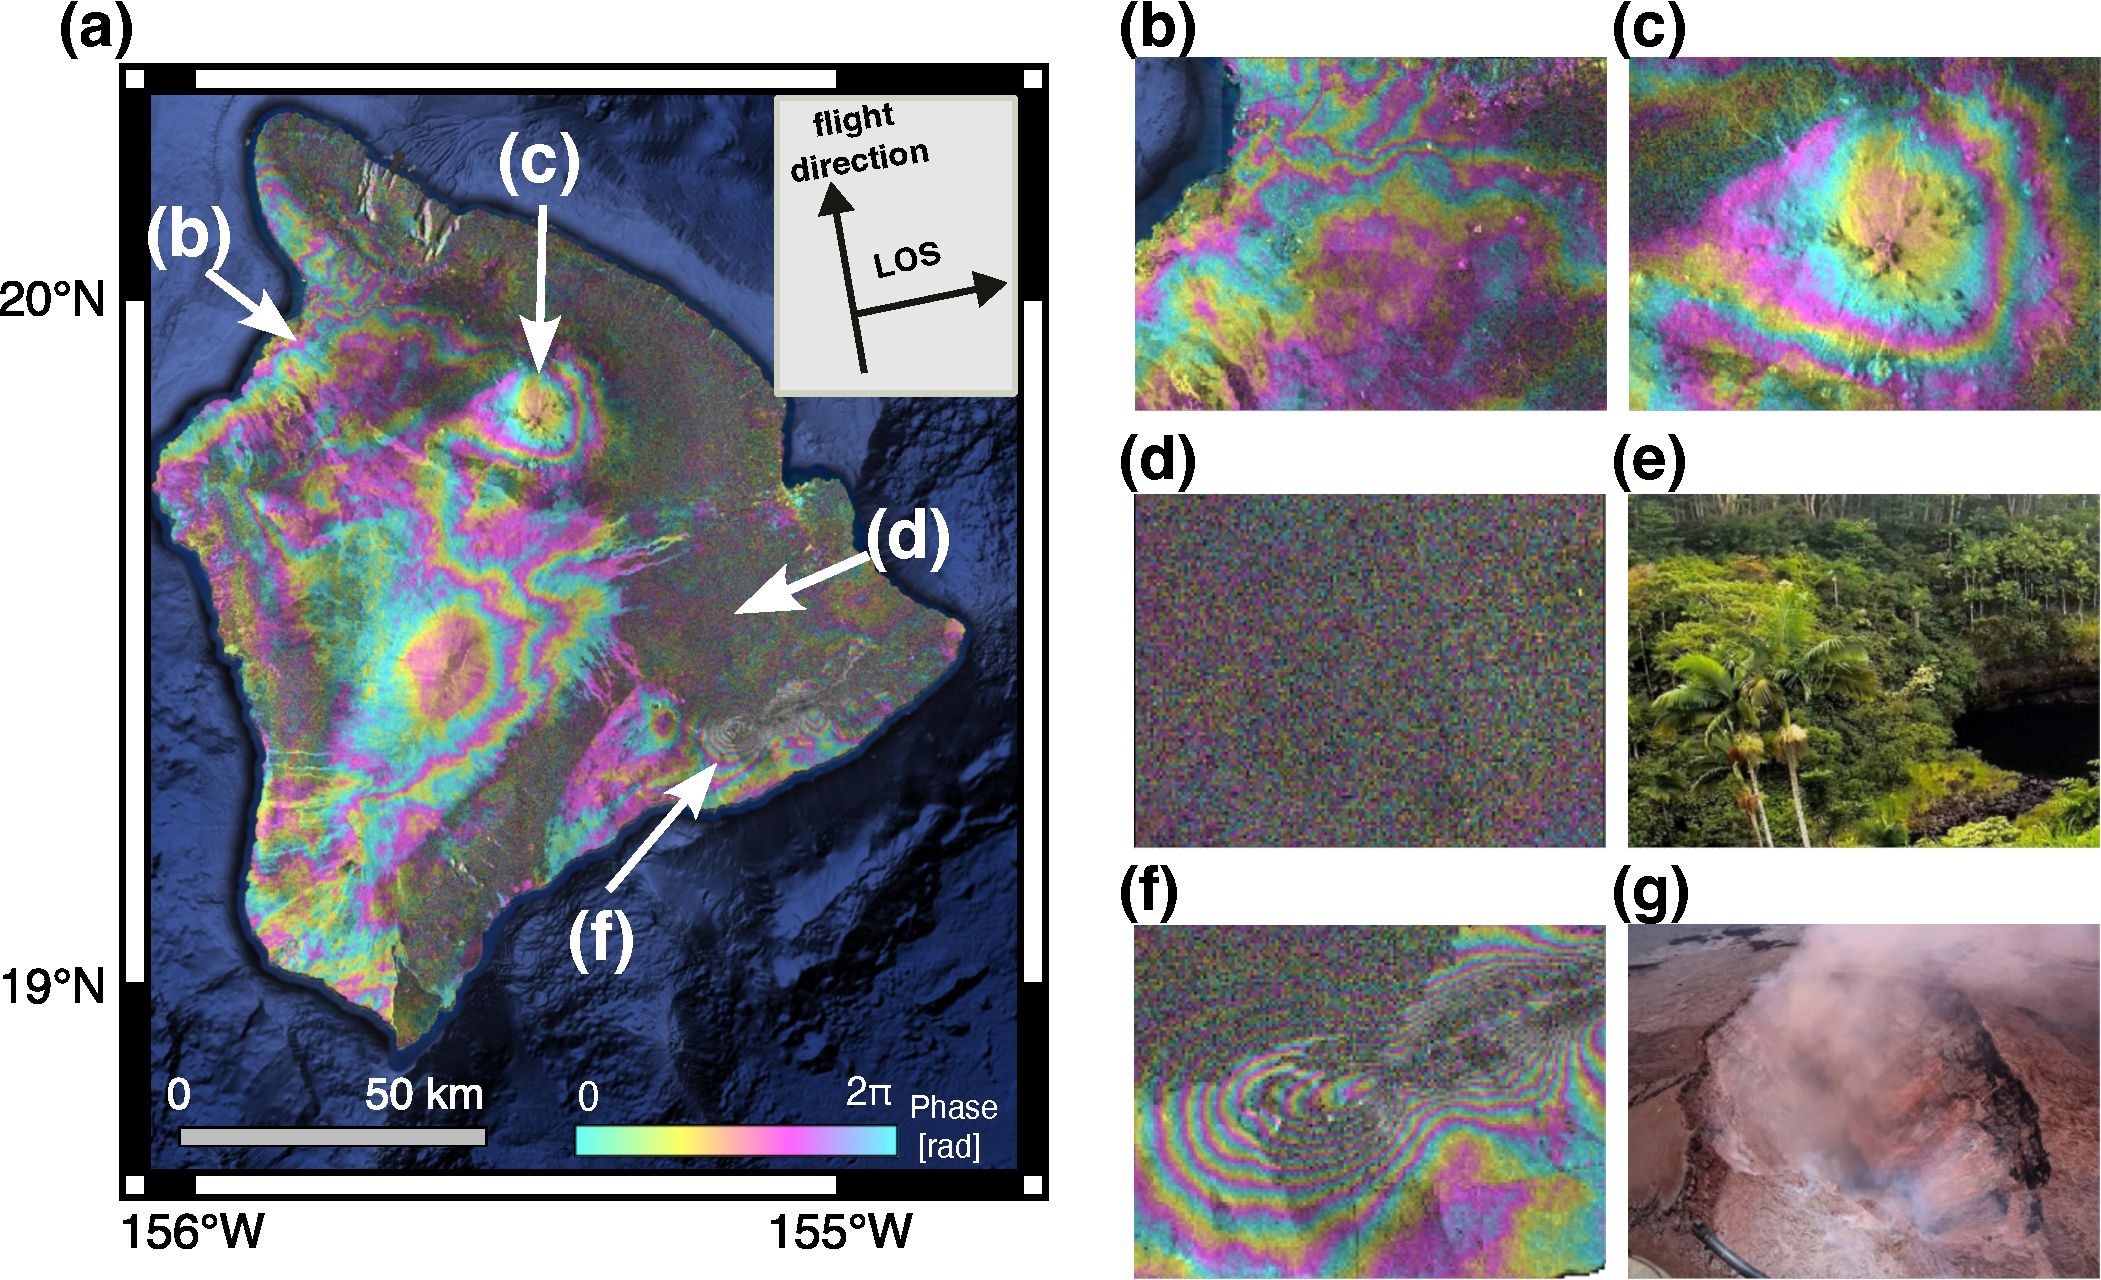
\includegraphics[width=1.0\textwidth]{figures/chapter3-sar/hawaii-example.pdf}
	\caption[Sentinel-1 interferogram over Hawaii showing common noise sources, along with 2018 eruption deformation]{
		(a) Sentinel-1 interferogram from April 20th, 2018 to May 2nd, 2018 over Hawaii, spanning the beginning of the 2018 eruption event.
		Each colored phase cycle of $2\pi$ radians indicates a range change of 2.7 cm along the radar line-of-sight, which can be caused by real surface deformation or a noise source.
		(b) The dense fringes near the coast are caused by turbulent tropospheric noise (see Section \ref{sec:ch3-noise-tropo-strat}).
		(c) Stratified tropospheric noise on the peak of Mauna Kea, the tallest peak on Hawaii at 4,207 m, causes a concentric ring pattern. This pattern is also visible on Mauna Loa in the center of the island, where the phase is strongly correlated with topographic height. See Section \ref{sec:ch3-noise-tropo-strat} for further details.
		(d) An example of decorrelation noise caused by dense tropical rain forests (e) located on windward side of the island.
		(f) Real deformation of $ \sim 40 $cm around the Pu'u '\=O'\=o volcanic cone to the east of K'\=ilauea. In this case, the ground was subsiding down and to the southeast as magma flowed away from Pu'u '\=O'\=o.
		%		The signal of interest in this interferograms, the collapse of the Pu'u '\=O'\=o caldera
		(g) An aerial photo of Pu'u '\=O'\=o shows the caldera collapse on April, 30th, 2018 after magma migrated eastward underground (image source: HVO / USGS).
	}
	\label{fig:sar-hawaii-example}
\end{figure}

Two days after the interferogram on May 4, a  M$_w$ 6.9 earthquake struck the south flank of the Lower East Rift Zone, just south of the zoom.


% at the Sentinel-1  The windward side of the island contains many dense tropical rain forests. These areas show Heavy decorrelation noise at the Sentinel-1 C-band wavelength of 5.5 cm.

%brief fissure eruption occurred on the west flank of the Puʻu ʻŌʻō cone on April 30, 20181. Over the next few days, earthquakes migrated eastward into the LERZ and rift-normal displacements were recorded by GPS instruments, signaling large-scale injection of magma downrift of Puʻu ʻŌʻō. Magma reached the surface in Leilani Estates subdivision on May 3, marking the onset of the LERZ eruption (Fig. 1a)

%1. Table: noise, specific to ifg or SAR, max variance?, common?


%2. Figure: Hawaii, showing Stratified, Turbulence, decorr, defo


%3. ? Figure: unwrap error? DEM error? iono noise? orb ramp?

\subsection{Tropospheric Noise}
\label{sec:ch3-noise-tropo}

%Ideas:
%
%- comparison of ways people have tried to correct for troposphere
%
%- plots/images of possible views into the single day atmosphere.
% -- modis
% -- HRRR, ECMWF
% --  GOES
% -- insar averaging
% 
% axes of comparison:
% - resolution
% - time availability
% - spatial availibility
% - sensitivity to phase propation delay
% 
% 
% SEASONAL plots...
% 

\subsubsection{Turbulent Tropospheric Noise}
\label{sec:ch3-noise-tropo-turb}

\subsubsection{Stratified Tropospheric Noise}
\label{sec:ch3-noise-tropo-strat}


Tropospheric noise in InSAR consists of a stratified component, which correlates with topography \citep{Doin2009CorrectionsStratifiedTropospheric}, and a turbulent component that is random at time scales longer than a day \citep{Emardson2003NeutralAtmosphericDelay, Onn2006ModelingWaterVapor}. Previous studies have made advances in correcting for the stratified component using global atmospheric models \citep{Doin2009CorrectionsStratifiedTropospheric, Jolivet2014ImprovingInsarGeodesy, Cao2021AdvancedInsarTropospheric}, GPS zenith delay measurements \citep{Onn2006ModelingWaterVapor}, external measurements from sensors such as the Moderate Resolution Imaging Spectroradiometer (MODIS) \citep{Li2005InterferometricSyntheticAperture, Barnhart2013CharacterizingEstimatingNoise} or the Medium Resolution Imaging Spectrometer (MERIS)  \citep{Ding2008AtmosphericEffectsInsar}, as well as empirical methods using regressions on InSAR phase and elevation \citep{Zebker2021AccuracyModelFree, Murray2021ClusterBasedEmpirical}.

Early efforts to correct or mitigate the turbulent atmospheric noise used a combination of high pass temporal filtering and low pass spatial filtering \citep{Ferretti2001PermanentScatterersSar, Berardino2002NewAlgorithmSurface}.
%- but as \citep{Liu2012SatelliteRadarInterferometry} notes, gaps in the acquistion, or strong non-Gaussianity from, e.g., severe thunderstorms, break the assumptions of equal variance among APS dates that these filters require.
Several research efforts have attempted to produce estimates of the atmospheric phase delay for each SAR acquisition directly from a time series of interferograms. \citep{Liu2012SatelliteRadarInterferometry} formulated the problem as a linear system using a network of small baseline interferograms. Since the problem of estimating both surface deformation and atmospheric delay is an ill-posed problem given only differential InSAR measurements, the authors assumed zero or known deformation of the study region, and they constrained the estimated troposphere to have zero mean. In an attempt to denoise time series of surface deformation, \citep{Tymofyeyeva2015MitigationAtmosphericPhase} averaged sets of redundant interferograms containing a common reference date, with an assumption of linear or slowly-varying deformation, and subtracted the estimated troposphere.

%  \citep{Havazli2021DetectionThresholdEstimates} almost does what i'm doing (with some type of stratified atmo too), it's just a random multiplier, and it looks like it was almost all simulation
An alternative approach to correcting for the tropospheric turbulence is to treat it as a stochastic noise source in time series analysis \citep{Simons2007InterferometricSyntheticAperture, Agram2015NoiseModelInsar} and estimate its covariance matrix either through auxiliary data sources \citep{Barnhart2013CharacterizingEstimatingNoise, Parker2015SystematicAssessmentAtmospheric} or directly from InSAR data \citep{Lohman2005SomeThoughtsUse}. While these approaches provide a measure of uncertainty in the deformation solution, the uncertainties are given for each pixel (or each model parameter), rather than for each visible deformation feature.




GACOS is an iterative tropospheric decomposition model that integrates global weather models and available GPS zenith delay measurements for estimating tropospheric noise in InSAR data \citep{Yu2018InterferometricSyntheticAperture}. Due to the limited spatial and temporal resolution of weather models and GPS data, GACOS is more effective in removing the stratified tropospheric noise \citep{Doin2009CorrectionsStratifiedTropospheric} than the random turbulent tropospheric noise \citep{Emardson2003NeutralAtmosphericDelay}. 
We found that GACOS does not produce substantial corrections in most Sentinel-1 West Texas interferograms for areas outside the main area of interest (e.g. Figure \ref{fig:GACOS} (a)-(c)). 

\textcolor{red}{Get an interferogram that works, and then show the one that doesn't}

\begin{figure}
	\centering
	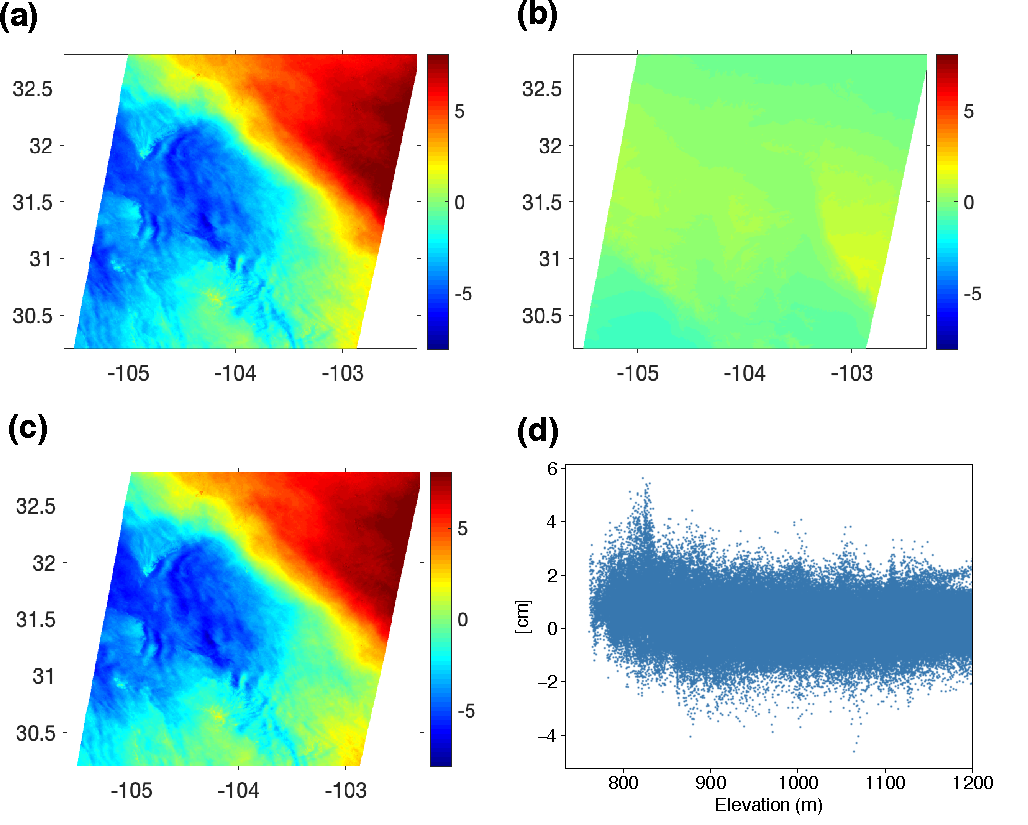
\includegraphics[width=\textwidth]{paper1-permian/figures/supplement/figureS4-gacos.pdf}		
	\caption[GACOS tropospheric corrections]{(a) LOS measurements (in cm) of a descending interferogram (20150127-20150220) before the GACOS correction. (b) GACOS tropospheric correction (in cm) for the 20150127-20150220 interferogram \citep{Yu2018InterferometricSyntheticAperture}. (c) LOS measurements (in cm) of a descending interferogram (20150127 - 20150220) after the GACOS correction. (d) LOS measurements (in cm) of the 20150127-20150220 interferogram vs. the Digital Elevation Model (DEM).}
	\label{fig:GACOS}
\end{figure}


\section{InSAR Time Series}
\label{sec:ch3-insar-ts}

stacking for avg rate

SBAS linear system. doesn't need to be short baseline. just a way to solve for the phase at each date

Phase linking approaches solve for this using an optimization on each pixels time-covariance matrix.


% Yunjun thesis: the vector of interferometric phase residual that does not fulfill the zero phase closure of interferogram triplets. It includes the decorrelation noise, phase contribution due to the change of dielectric properties of ground scatterers such as soil moisture (De Zan et al., 2014; Morrison et al., 2011), processing inconsistency such as filtering, multilooking, coregistration and interpolation errors (Agram and Simons, 2015; Hanssen, 2001), and/or phase-unwrapping errors.

%An alternative objective function to solve equation (2.1) is minimizing the L2-norm of the residual of phase velocity of adjacent acquisitions (equation (16) in Berardino et al. (2002)). Optimizations with both objective functions give nearly identical solutions for a fully connected network


\subsection{Uncertainty}
\label{sec:ch3-eq-tropo}
Several ways for uncertainty.

jackknife (maybe look into the NSBAS/GIANT time series way they do it....). prob an underestimate, since this is *precision* of the estimator. often it's jsut precision of the noise+deformation phase. but we really want the defo phase.

other is least squares propagation of covariance. difficult to calibrate without good atmo noise estimate, can underestimate/overestimate.

one problem with daily time series: often uncertainty is a single number. but each day's atmo noise can vary by 10-20x.

Even with temporal smoothing (example pic of that super storm cell), there can be many days with "blobs" of atmospheric noise which exceed real deformation.

Chapter (2nd paper) will discus a third novel way using computer vision.


Bootstrap:

From "practictioners guide":
A natural question for the practitioner is to ask  “ Why bootstrap in the linear regression case? Isn ’ t least - squares a well - established approach that  has  served  us  well  in  countless  applications? ”   The  answer  is  that  for  many  problems, least - squares regression has served us well and is always useful as  a first approach but is problematic when the residuals have heavy - tailed distributions or if even just a few outliers are present.

IID assumption: doesn't hold for time series... still gives some estimate. maybe show example of how it overestimates, but that it's not bad because it's mostly accounting for tropo, and not for the phase UQ (cite Zwiebeck paper).


%Problems with pixelwise
%- Image of blob, with 8 mm cutoff, question which part you trust and not
%- Leads into feature-wise uq



\section{InSAR Line-of-sight Decomposition}
\label{sec:ch3-insar-decomp}
An interferogram measures surface deformation between the two SAR acquisition times along the radar line-of-sight (LOS) direction. The LOS deformation, $u_{LOS}$, can be written as: 
\begin{align}
	u_{LOS}= \alpha_{e} u_{e} + \alpha_{n} u_{n} + \alpha_{u} u_{u}
\end{align}
where $u_{e}$, $u_{n}$ and $u_{u}$ are the east, north and up displacements, respectively. The radar look vector $\alpha = [\alpha_e, \alpha_n, \alpha_u]$ can be calculated from the known imaging geometry at every pixel location. This varies significantly across the basin due to the $ \sim$250 km wide Sentinel swath (Figure \ref{fig:los-map}). 


%
%\begin{figure}
%	\centering
%	% TODO
%	%	\includegraphics[width=\textwidth]{}
%	\caption[Line of sight convention]{Line of sight convention used in this thesis for ascending (a) and descending (b) satellite geometries. Vector points from the satellite to the ground}
%	\label{fig:los-asc-desc}
%\end{figure}

\begin{figure}[!htbp]
	\centering
	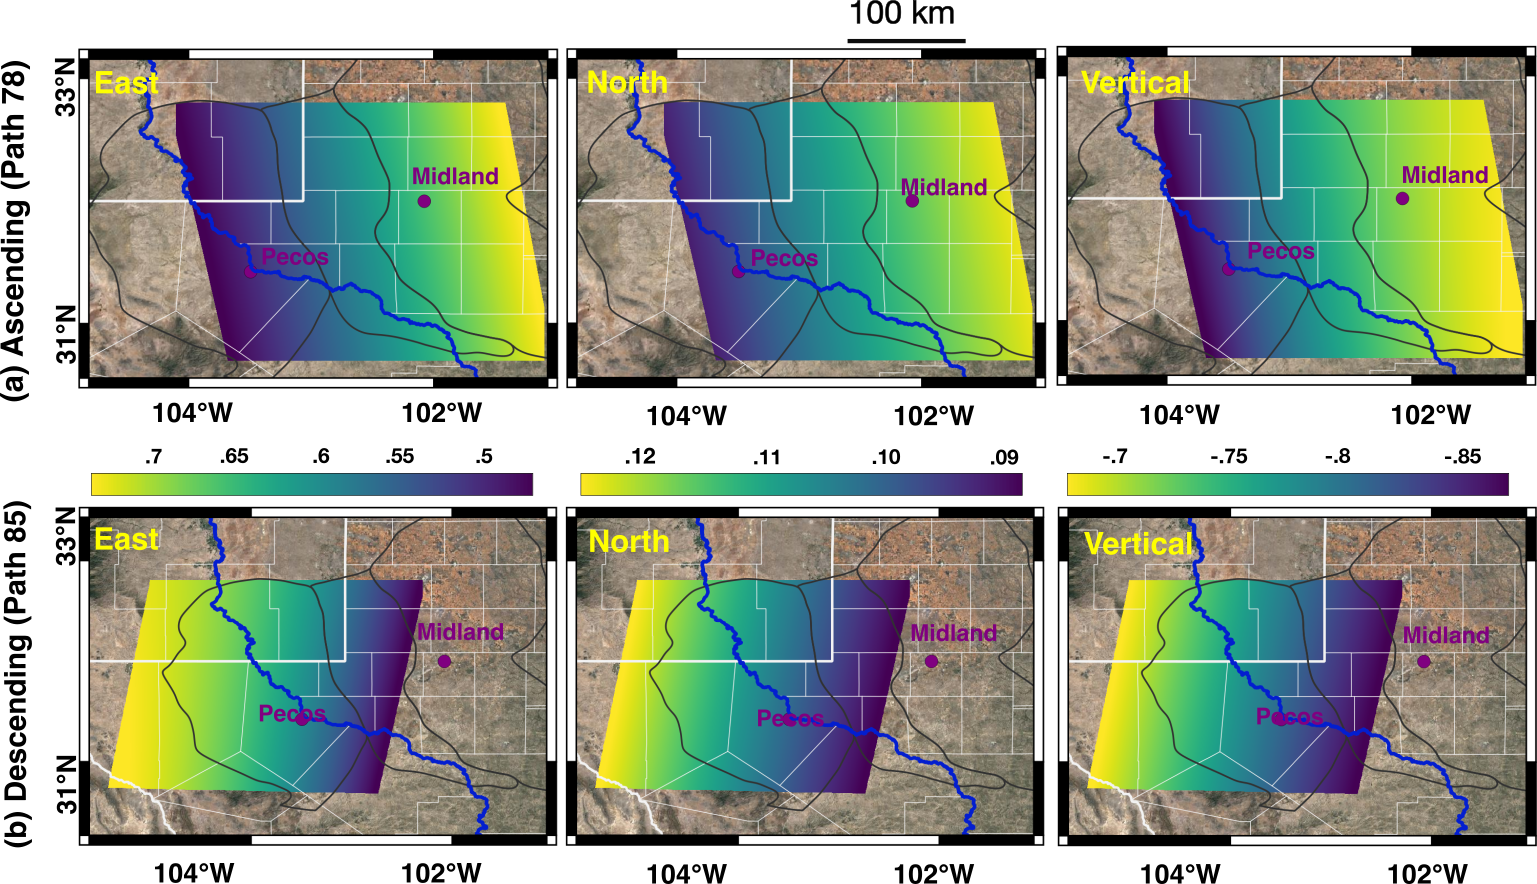
\includegraphics[width=.98\textwidth]{paper1-permian/figures/supplement/figureS2-los.pdf}
	\caption[East, north, and vertical coefficients of Sentinel-1 LOS vectors]{East, north, and vertical coefficients of the LOS unit vector of all Sentinel-1 path 78 and path 85 pixels. Positive LOS direction points away from the satellite to the ground.}
	\label{fig:los-map}
\end{figure}

In regions where InSAR data are available from two LOS directions, we can decompose the ground motion into its eastward and vertical components.
To perform the decomposition, we first write $u_{asc}$ and $u_{desc}$ in terms of $u_e$, $u_n$ and $u_u$:
\begin{align}
	u_{asc} &= \alpha_{a,e} u_{e} + \alpha_{a,n} u_{n} + \alpha_{a,u} u_{u}\\
	u_{desc} &= \alpha_{d,e} u_{e} + \alpha_{d,n} u_{n} + \alpha_{d,u} u_{u}
\end{align}
We can express $u_e$ and $u_u$ as:
\begin{align}
	u_{e} &\approx  \frac{1}{\beta}  \left[\alpha_{d,u}  u_{asc} - \alpha_{a,u} u_{desc} \right] \\
	u_{u} &\approx  \frac{1}{\beta}  \left[\alpha_{a,e} u_{desc} - \alpha_{d,e}  u_{asc}  \right] 
\end{align}
where  $ \beta = {\alpha_{a,e} \alpha_{d,u}- \alpha_{d,e} \alpha_{a,u}} $.

Because Sentinel-1 satellites are operating in a near-polar orbit, the north look coefficients $\alpha_{a,n}$ and $\alpha_{d,n}$ are both relatively small. Ignoring 1 cm northward motion in $u_n$ only leads to $\sim$ 0.1-0.2 mm error in $u_e$ and $\sim$ 1 mm error in $u_u$ at most locations. \cite{Kim2018AssociationLocalizedGeohazards} detected several localized deformation features within the Delaware Basin related to wastewater injection, CO2 injection, and hydrocarbon production using Sentinel-1 InSAR data.  Our LOS decomposition results are consistent with their study at these locations. For example, in a 12 km x 12 km region centered on a wastewater injection well, we observed $\sim$ 5.5 cm of uplift and $\sim$1.2 cm of east-west motion between November 2014 and April 2017 (Figure \ref{fig:injection-kim-lu}). 



\begin{figure}
	\centering
	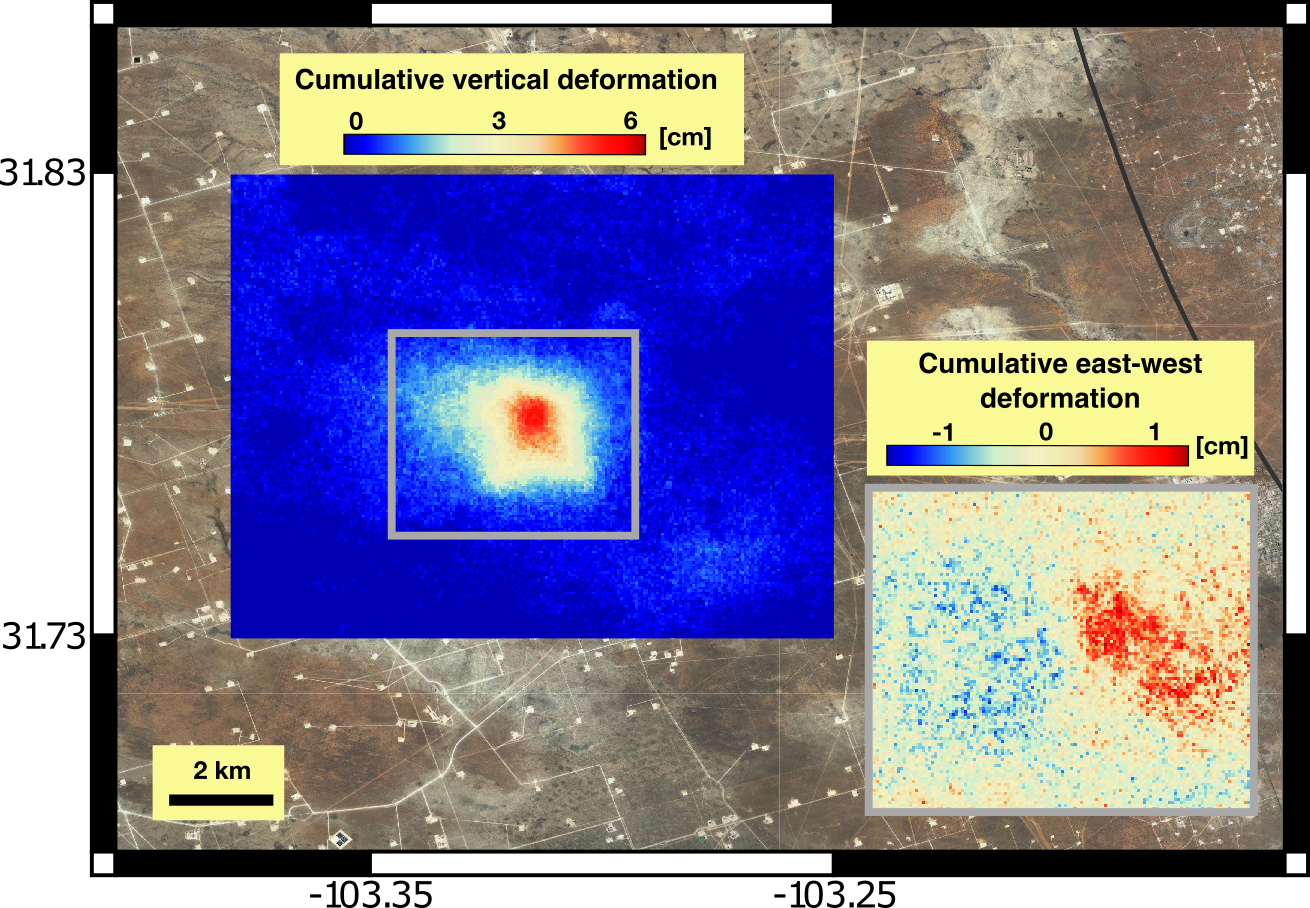
\includegraphics[width=\textwidth]{paper1-permian/figures/supplement/figureS3-injection-kim-lu.pdf}
	\caption[Vertical and horizontal deformation near Winkler County, TX]{Cumulative surface deformation between November 2014 and April 2017 due to wastewater injection in Winkler County, TX. The horizontal motion here is $\sim$ 20\% of the vertical motion, with up to $\sim$ 5.5 cm of uplift and $\sim$ 1.2 cm of east-west motion. This localized deformation feature was originally reported in \cite{Kim2018AssociationLocalizedGeohazards}.}
	\label{fig:injection-kim-lu}
\end{figure}




\subsection{Uncertainty Propagation through LOS decomposition}
\label{sec:ch3-decomp-uq-prop}
Since the LOS decomposition is a linear operation, given two LOS uncertainties, we can use linear uncertainty propagation theory to determine the vertical/horizontal uncertainties.

TODO: move this to appendix or not?


